\begin{comment}
\subsection{Distributed-prover Zero-knowledge Protocols}
This discussion will formally define a zero-knowledge protocol which supports multiple proves and distributed proof generation.
\subsubsection{Definition of DPZK}
Consider a language $L \in \npol$ and the corresponding relation $R \in \pol$  \commentA{what is $\pol$} such that
\[
\stmt \in L \Leftrightarrow R(\stmt, \wit)=1 \text{ for some witness } \wit
\]
Let $\prover_1, \ldots, \prover_{\Num}$ be $\Num$ provers. In our setting, we let each party have an additive share of the witness $\wit$. For prover $i \in [\Num]$, let $\wit_i$ be its share.  The witness $\wit$ and its shares have length equal to the number of input wires of the circuit $\C$ representing the relation $R$. We will discuss later in this section why we decided to do an additive share of the witness. \commentA{the following didn't make sense to me}For now, note that a partition of the witness among the provers such that each prover owns a non-intersecting piece of the witness is a sub-class of additive sharing since the share of a prover can be its partition of the witness padded with zeros in the rest of positions.


A DPZK protocol consists of three probabilistic polynomial time algorithms: $(\setup, \Pi, \verifier)$. 
\begin{itemize}
\item $\setup$ takes as input the security parameter $1^\secp$ and optionally a trapdoor $\tau$ and outputs the public parameters $\sigma$ of the system.
\item The interactive proof system is an $\round$-round protocol $\langle \Pi = \{\pi_i\}_{i \in [\round]}, \verifier \rangle$ where in every round $i \in [\round]$, we have the output $m_i$ of $\pi_i(\st^i_1, \ldots, \st^i_{\Num})$ provided to $\verifier$. Here, $\st^i_j$ is the state of the prover $\prover_j$ at round $i$. $\st^1_j$ is set to $\prover_j$'s share of the witness $\wit_j$, randomness $r_j$, the public parameters $\sigma$ and updated later as the protocol proceeds. The output of $\verifier$ is either an $\tt accept$ (1) or a $\tt{reject}$ (0). Also, let $\tr$ be the transcript of the protocol.
\end{itemize}
A $\DPZK$ protocol for a language $L$ satisfies the following properties: 
correctness, soundness, zero-knowledge and privacy among provers.


\begin{comment}
\begin{myboxfig}{Ideal Functionality for Distributed ZK}{funcsabort}
	\begin{center}
		\textbf{ $\FDPZK$}
	\end{center}
	%Each honest party $P_i$ sends its input $x_i$ to the functionality. Corrupted parties may send the trusted party arbitrary inputs as instructed by the adversary. When sending the inputs to the trusted party, the adversary is allowed to send a special $\abort$ command as well.
	\begin{description}
	\item[--] $ $
	%	\item[\textbf{Input:}] On message $(\sid,\In, x_i$) from a party $P_i$ $(i \in [3])$, do the following: if $(\sid,\In, *)$ message was received from $P_i$, then ignore. Otherwise record $x_i' = x_i$ internally. 	If $x_i'$ is outside of the domain for $P_i$ $(i \in [3])$, consider $x_i' = \abort$. 
		
	%	\item[\textbf{Output to adversary:}] If there exists $i \in [3]$ such that $x_i' = \abort$, send $( \sid,\Output, \bot)$ to all the parties. Else, send $(\sid,\Output, y)$ to the adversary, where $y = f(x_1', x_2', x_3')$.
		
	%	\item[\textbf{Output to selected honest parties:}] 	Receive $(\select, \{I\})$ from adversary, where $\{I\}$ denotes a subset of the honest parties. %(where $\{I\}$ may denote empty set or ). If an honest party belongs to $I$, send $(\sid,\Output, y)$, else send $(\sid,\Output, \bot)$. 
		
		%		If there exists $i \in [3]$ such that $x_i' = \abort$, send $( \sid,\Output, \bot)$ to all the parties. Else, send $(\sid,\Output, y)$ to the corrupt party $P^*$, where $y = f(x_1', x_2', x_3')$.
		
	\end{description}
\end{myboxfig}

\commentA{I discussed with protik yesterday, it's better to change this to rael/ideal world setting.}
\dnote{self: give a name for Privacy among provers}
\paragraph{Completeness}: %We will define correctness assuming that the witness set is minimal.
Given $\sigma \gets \Setup(1^\secp, \tau)$ and a valid witness $\wit$ corresponding to $\stmt \in L$, when the initial states are set with $\sigma$ and the shares of $\wit$, $\langle \Pi, \verifier \rangle$ outputs 1 with probability 1.

\paragraph{Soundness}:  The basic definition of soundness ensures the existence of a valid witness for $\stmt \in L$. For every instance $\stmt \notin L$ and any $\ppt$ algorithm $\Pi^*$, $\verifier$ accepts with probability at most $\negl(\secp)$.

The notion of proof of knowledge of the witness by the prover is captured by the notion of knowledge extraction where an extractor extracts the witness whenever the verifier accepts using an oracle access to the prover. The stronger notion of witness extended emulation \cite{Lindell03} proposes the existence of an emulator which additionally produces a simulated transcript between the prover and the verifier irrespective of whether the verifier accepts or not. We will now define the notion of witness-extended emulation for the $\DPZK$ setting, adapted from \cite{Groth11}. 
%\commentA{I do not understand the below definition; two probabilities are indistinguishable? why is $\adv$ outputting one goven $\tr$???? same with remaining definitions}
\begin{definition}
The argument $(\Setup, \Pi, \verifier)$ has computational witness-extended emulation if for all deterministic polynomial time $\Pi^*$ there exists an expected polynomial time emulator $\chi$ such that for all non-uniform polynomial time adversaries $\adv$ and all $\tau$
\begin{align*}
& \pr \left[\sigma \leftarrow \Setup(1^\secp, \tau); (\stmt, \{\wit_i\}_{i \in [\Num]}) \leftarrow \adv(\sigma); \tr \leftarrow \langle \Pi^*, \verifier \rangle: \adv(\tr) = 1 \right] \\
\approx \; & \pr \left[\sigma \leftarrow \Setup(1^\secp, \tau); (\stmt, \{\wit_i\}_{i \in [\Num]}) \leftarrow \adv(\sigma); (\tr, \wit) \leftarrow \chi^{\langle \Pi^*, \verifier \rangle}(\sigma, x): \right. \\
&\;\;\; \adv(\tr) = 1 \left. \text{ and if } \tr \text{ accepts then } \stmt \in L \text{ with } \wit \text{ as witness} \right] 
\end{align*}

where $\chi$ has access to the oracle $\langle \Pi^*, \verifier \rangle$ which produces the transcript. $\chi$ can rewind $\langle \Pi^*, \verifier \rangle$ to any round and resume the protocol with fresh randomness from the verifier.
\end{definition}
%.\dnote{1. should the notation $\langle \Pi, \verifier \rangle$ be modified to also take their respective inputs?\\
%2. Proof of knowledge \textit{vs} argument of knowledge}
Note that this follows from the single prover definition since an adversarial prover in the single prover definition can be any $\ppt$ algorithm, and this is independent of whether the $\ppt$ algorithm is run by a single prover or a protocol between multiple provers.
Also, allowing for any adversarial $\Pi^*$ captures adversarial behaviour by all the parties.

\paragraph{Zero-knowledge}: 
The traditional notion of zero-knowledge ensures that the proof does not reveal any information beyond the fact that the instance is in the language.
This is a property with respect to the view of the verifier $\verifier$. The protocol $\Pi$ and the number of provers involved to produce these messages do not impact the zero-knowledge property. The following definition captures this formally.
\begin{definition}
The argument $(\Setup, \Pi, \verifier)$ is a special honest verifier zero-knowledge argument for $L$ if there exists a PPT simulator $S$ such that for all non-uniform polynomial time adversaries $A$ and all $\tau \in \secp^{O(1)}$ 

\begin{align*}
&\pr [\sigma \leftarrow \Setup(1^\secp, \tau); (\stmt ,\wit ,\rho) \leftarrow \adv(\sigma); \tr \leftarrow \langle \Pi, \verifier_\rho \rangle:\\
 &\stmt \in L \text{ with witness } \wit \text{ and } \adv(\tr)=1 ]\\
\approx \; &\pr [\sigma \leftarrow \Setup(1^\secp, \tau); (\stmt,\wit,\rho) \leftarrow \adv(\sigma); \tr \leftarrow S(\sigma,\stmt,\rho):\\ &\stmt \in L \text{ with witness } \wit \text{ and } \adv(\tr) = 1 ]
\end{align*}
\end{definition}
%.\dnote{Auxiliary input zk or just without it?}

\paragraph{Zero Knowledge under $t$-collusions}: 
The notion of zero-knowledge, as we discussed earlier, considers the knowledge gained by a verifier on seeing the proof. However, when there are multiple provers, this does not capture the setting where the verifier colludes with a subset of provers trying to learn information about the witness shares of the remaining provers. We define the notion of zero-knowledge under $t$-collusions ($t$-$\ZKUC$) to capture this.

\begin{definition}
An argument $\innp{\Pi}{\verifier}$ with $\Num$ provers has the property of computational zero-knowledge under $t$-collusions ($t$-$\ZKUC$), if for every $\ppt$ interactive machine $\verifier^*$ and any subset of colluding provers $T\subseteq [\Num]$ of size $\leq t$, there exists a $\ppt$ algorithm $\Sim$ such that the following holds for any instance $\stmt \in L$ with witness $\wit$ and for any $\rho$: 
\[
 \{ \innp { \prover_{\overline{T}}( \st^{i-1}_{\overline{T}} ) } { \prover_T ( \st^{i-1}_T ) } ( \stmt  , m_i): i\in [\round] \} \cup \innp{\Pi(\stmt, \wit)}{\verifier^*(\stmt, \rho, \wit_T)}  \stackrel{c}{\approx}  \Sim (\stmt, \rho)
\]
where in the malicious setting, $\Sim$ has access to the ideal functionality $\IF{DPZK}$ that outputs 1 or 0 according to the extracted input of the corrupt parties, and in the semi-honest setting, $\Sim$ has input, $\wit_T$, of the corrupt parties and output of the execution.
$\st^{i-1}_T$ consists of the states of the corrupt parties of $i$th round and $\st^{i-1}_{\overline{T}}$ consists of the states of the honest parties of $i$th round. 
\end{definition}

.\pnote{Define this notion for malicious adversary}
\end{comment}
%------------------------------------------------------------------------------------------------
% Functionality based definition:
\section{The  Security Model and Definition}\label{sec:security model}
We prove the security of our protocols based on the standard real/ideal world paradigm.  Essentially, the security of a protocol is analyzed by comparing what an adversary can do in the real execution of the protocol to what it can do in an ideal execution,  that is considered secure by definition (in the presence of an incorruptible trusted party). In an ideal execution, each party sends its input to the trusted party over a perfectly secure channel, the trusted party computes the function based on these inputs and sends to each party its respective output.  Informally, a protocol
is secure if whatever an adversary can do in the real protocol (where no trusted party exists) can be done in the above described ideal computation. We refer to \cite{Canetti00,Goldreich2001,Lindell17,CohenL14} for further details regarding the security model.  


\paragraph{The ideal Execution.} The ``ideal" world execution of DPZK  involves parties in $\Partyset$ that includes $\Num$ provers $\{\prover_1, \ldots, \prover_{\Num}\}$ and a verifier $\verifier$,  an ideal adversary $\Sim$ who may corrupt various subset of parties in $\Partyset$, and a  functionality $\Func_{\DPZK}$.  The functionality is parametrized with an  NP language $L$ and  the corresponding relation/verification function $R$. Each prover $\prover_i$ sends $(\stmt,\wit_i)$ to $\Func_{\DPZK}$, where $\stmt$ is the statement and $\wit_i$ is the $i$th part of the witness. The verifier $\verifier$ sends $x$.  $\Func_{\DPZK}$ computes $\wit = \wit_1 \oplus \wit_2,\ldots,\oplus \wit_\Num$, where $\oplus$ is the combining function of the parts of the witness held by the provers distributedly, and sends $R(\stmt,\wit)$ to $\verifier$ and $\bot$ to every $\prover_i$. $\Func_{\DPZK}$  is described below. 
\begin{figure}[H]
	\centering
	\begin{framed}
		\textbf{Functionality} (The Distributed Prover Zero Knowledge Functionality $\Func_{\DPZK}$)
		The functionality is parameterized with an NP relation $R$ of an NP language $L$.
		\begin{itemize}
		\item[--] Upon receiving input $x_i = (\stmt, \wit_i)$ from $\prover_i$ $\forall i\in[\Num]$ and $\stmt$ from $\verifier$, do the following: if $x_i$ is an empty string or falls outside the range of the domain of $\prover_i$'s input,  reset $x_i = \abort$. 
			\item[--] If any of the $x_i$ is $\abort$ send $\abort$ to everyone in $\Partyset$. Otherwise,   compute $\wit = \wit_1 \oplus \wit_2,\ldots, \oplus \wit_\Num$, where $\oplus$ is the combining function of the parts of the witness held by the provers distributedly and send $R(\stmt, \wit)$ to $\verifier$ and $\bot$ to everyone else. 
		\end{itemize}
	\end{framed}
	\caption{Ideal Functionality $\Func_{\DPZK}$}
\end{figure} \label{func:DPZK}

Let the corrupt set be denoted as $I$. We let $\Ideal_{\Func_\DPZK, \Sim(z),I}(\vec{x})$ denote the random variable consisting of the output pair of the honest parties and the ideal-world adversary $\Sim$ controlling the corrupt parties in $I$ upon inputs $\vec{x} = (x_1  ,\ldots,x_{\Num},x_\verifier)$ for the parties and auxiliary input $z$ for $\Sim$.  


\paragraph{The Real world.} The ``real" world execution involves the $\ppt$\ parties  in $\Partyset$,  and a real world adversary $\Adv$ who may corrupt  $t$ of the parties.  Similarly,  let $\Real_{\Pi, \Adv(z),I}(\vec(x))$ denote the random variable consisting of the output pair of the honest parties and the adversary $\Adv$ controlling the corrupt parties in $I$ in the real execution, upon inputs $\vec{x}$ for the parties and auxiliary input $z$ for $\adv$. 




\begin{definition}
	Let $\Func$ be a functionality and let $\Pi$ be a $n$-party protocol involving $\Partyset$. We say that  $\Pi$ {$\it$ perfectly-securely realizes} $\Func$~if for every probabilistic  real world adversary $\Adv$, there exists a ideal world adversary $\Sim$ of comparable complexity, such that for every $I \subset \Partyset$ of cardinality at most $t$, every $\vec{x} \in (\{0,1\}^*)^n$ where $\abs{x_1} = \ldots= \abs{x_n}$, and every $z \in \bit^*$, it holds that:
	
	$$\Big\{\Ideal_{\Func, \Sim(z),I}(\vec{x}) \Big\} \equiv \Big\{ \Real_{\Pi, \Adv(z),I}(\vec{x}) \Big\}. $$
\end{definition}
%.\pnote{Change from IT to computational}
For computational security, the adversaries are defined to be $\ppt$, the adversaries are parametrised with a security parameter $\secparam$ and the perfect indistinguishability is replaced with computational indistinguishability. 
%\paragraph{\bf The $\Func$-hybrid model.}
%In order to construct some of our protocols, we will use secure two-party protocols as subprotocols. The standard way of doing this is to work in a ``\emph{hybrid model}'' where both the parties interact with each other (as in the real model) in the outer protocol and use ideal functionality calls (as in the ideal model) for the subprotocols. Specifically, when constructing a protocol $\Pi$ that uses a subprotocol for securely computing some functionality $\Func$,  the parties run $\Pi$ and use ``ideal calls'' to $\Func$ (instead of running the subprotocols implementing $\Func$). %Upon receiving the inputs from the parties, $\F$ will return all parties their output. Then, after receiving these outputs back from $\F$, the protocol $\Pi$ continues.
%The execution of $\Pi$ that invokes $\Func$ every time it requires to execute the subprotocol implementing $\Func$ is called   the {\em $\Func$-hybrid execution of $\Pi$} and is denoted as $\Pi^\Func$. The hybrid ensemble $\Hyb_{\Pi^\Func,\Adv,\Env}(1^\secparam,z)$ describes $\Env$'s output after interacting with $\Adv$ and the parties $P_0$, $P_1$ running protocol $\Pi^\Func$. By UC definition, the hybrid ensemble should be indistinguishable from the real ensemble with respect to protocol $\Pi$ where the calls to $\Func$ are instantiated with a realization of $\Func$.
%-----------------------------------------------------------------------------------------------
\subsection{Distributed-prover Zero-knowledge Protocols}
%-In this section we will describe the notion of distributed proof generation for zero-knowledge and the adversarial model.

\noindent We will model this distributed proof generations for zero-knowledge in the same way described in above section ~\ref{sec:security model}. Here $\Partyset$ consists of $\Num$ provers $\{\prover_1, \ldots, \prover_{\Num}\}$ and a verifier $\verifier$. For some NP language $L$ and instance $\stmt$ of $L$, parties in $\Partyset$ involves in a protocol $\innp{\Pi}{\verifier}$ so that all the provers in $\Partyset$ convince the verifier that there is a witness $\wit$ such that the deterministic verification algorithm $R$ for $L$ outputs $R(\stmt,\wit) = 1$, and claim of the prover is that $\prover_i$ has $\wit_i$, for all $i\in[\Num]$ such that $\wit = (\wit_1, \ldots, \wit_{[\Num]})$. Therefore the funcitonality is as follows: 
\begin{figure}[H]
	\centering
	\begin{framed}
		\textbf{Functionality} (The Distributed Prover Zero Knowledge Functionality $\Func_{\DPZK}$)
		\begin{itemize}
			\item[--] The functionality is parameterized with an NP relation $R$ of an NP language $L$.
			\item[--] Upon receiving input $(\stmt, \wit_i)$ from $\prover_i$ $\forall i\in[\Num]$, check that $R(\stmt, (\wit_1, \ldots, \wit_{[\Num]})) = 1$. If so send 1 to the verifier $\verifier$, else send 0. 
		\end{itemize}
	\end{framed}
	\caption{Ideal Functionality}
\end{figure} \label{func:DPZK}
In contrast to the definition in section ~\ref{sec:security model}, all the parties except for the verifier, in the execution of the protocol they may deviate arbitrarily, but the verifier is not allowed to deviate from the protocol. The reason behind considering a preposterously looking adversarial model is that we want to design a zkSNARK which is efficient, secure, publicly verifiable and distributed proof generation property. We know from \cite{}, any interactive honest (public coin) verifier can be transformed into Non-interactive zero-knowledge using \textit{Fiat–Shamir heuristic}. Here the verifier can be semi-honest, i.e., verifier will follow the protocol steps and sends all the challenges uniformly at random.
%-Start with corruption model and give a brief reasoning.
%.\pnote{Describe honest verifier}

If all the parties in $\Partyset$ are honest, then the protocol should return 1, this property is called \textbf{\textit{completeness}}.

In this setting, we have two types of corruption models, and that depends on which parties are corrupt:
\begin{itemize} 
	\item Consider $I$, the set of all corrupt parties consists of all the provers in $\Partyset$, i.e., together they do not have a correct witness for $\stmt$, but they try to cheat in such a way so that the verifier outputs 1. What we want from the protocol is that such a scenario can happen with negligible probability. In other word, whenever in the protocol $\verifier$ outputs 1, then there must be a correct witness $\wit$ such that $\prover_i$ has $\wit_i$ for which $\wit = (\wit_1, \ldots, \wit_{\Num})$, with very high probability. This notion is called \textbf{\textit{proof of knowledge}}. 
	\begin{definition}
		Let $\Func_{\DPZK}$ is the functionality which is defined as ~\ref{func:DPZK} and let $\innp{\Pi}{V}$ is a $\DPZK$ $\Num$-party protocol involving $\Partyset$. We say that $\innp{\Pi}{V}$ realizes $\Func_{\DPZK}$ with computational proof of knowledge property if for every $\ppt$ real world adversary $\Adv$, corrupting at most all provers, there exists a $\ppt$ knowledge extractor $\extrac$ such that for every $\stmt \in L$, for which $\verifier$ outputs 1, $\extrac$ can extract a witness $(\wit_1, \ldots, \wit_{\Num})$ for which $\Func_{\DPZK}$ outputs 1.
	\end{definition}    
	
	\item Consider $I$ consists of $\verifier$ and $t$ provers. That is, some of the provers may deviate from the protocol to gain additional information about the honest provers' secret; to achieve this, they may take additional help from $\verifier$'s view. We call a protocol $\innp{\Pi}{\verifier}$ has \textbf{\textit{zero knowledge under t-collusion}}($t$-ZKUC) property, if in this corruption model, corrupted provers and verifier whatever they can compute, the same thing can be computed from the functionality output of the functionality. 
	\begin{definition}
		Let $\Func_{\DPZK}$ is the functionality which is defined as ~\ref{func:DPZK} and let $\innp{\Pi}{V}$ is a $\DPZK$ $\Num$-party protocol involving $\Partyset$. We say that $\innp{\Pi}{V}$ realizes $\Func_{\DPZK}$ with computational zero knowledge under $t$-collusion property if for every $\ppt$ real world adversary $\Adv$, corrupting $I$, at most $t$ provers and verifier, then there exists a $\ppt$ simulator $\Sim$ such that for every $\stmt$, and $\{\wit_i : i\in [\Num]\}$, it holds that: 
		$$\Big\{\Ideal_{\Func_{\DPZK}, \Sim(\secparam),I}(\wit_1, \ldots, \wit_{\Num}) \Big\} \stackrel{c}{\approx} \Big\{ \Real_{\innp{\Pi}{\verifier}, \Adv(\secparam, \wit_T),I}(\wit_1, \ldots, \wit_{\Num}) \Big\}. $$
		Where $\wit_T$ is the input of the corrupt parties.
	\end{definition}
\end{itemize}

Note that if $I$ consists of the only verifier, then the view of the verifier should not reveal any information about neither the witness nor the inputs of the provers. This notion is called \textbf{\textit{zero knowledge}}, which is subsumed by the notion $t$-ZKUC.

\subsection{Strongly Private DPZK}
Here we will define a notion which is strictly stronger than the scenario when the some the provers are corrupt; we will call it \text{strongly private} DPZK, if it has the property that each interaction among the prover is simulatable separately and there is an outer simulator which can simulate each of the interaction.

We will show that some of the constructions that we are presenting this paper it satisfy this property, and we will prove in theorem ~\ref{theo:equivalent} that this stronger notion of privacy together with zero-knowledge property is as strong as zero-knowledge under collusion.

This notion can be defined for both semi-honest and malicious corruption models; in our work, we will present \textit{strongly private} DPZK protocols under semi-honest corruption.

%This notion captures the privacy of a prover's share of witness from other provers. The provers interact to generate shares of the extended witness $\extwit$ and then to compute the messages to be sent to the verifier. The privacy notion here can be formalized as multi-party computation protocols among the provers. The transcript of the interaction between provers can be simulated by a simulator with access only to the secret inputs of the corrupted provers and the final output of the interaction. Hence, for a protocol supporting $t$ corruptions, the input witnesses of the remaining honest prover cannot be inferred by an adversary possessing the inputs and controlling the actions of these $t$ provers.
%\dnote{ include formal definition}
%Whenever provers interact, there is a simulator with access to corrupt provers' input and output of the interaction can generate a transcript which is indistinguishable (computationally) from a real transcript. 

\begin{definition}
	Let $T\subseteq [\Num]$ be the set of corrupt parties and let $m_i$ be the output of $\Exec^{\pi_i}(\st^i_1, \ldots, \st^i_{\Num})$. An argument $\innp{\Pi = \{\pi_i\}_{i \in [\round]}}{\verifier}$ with $\Num$ provers has $t$-privacy if for any $T$ of size $\leq t$, there is a $\ppt$ simulator $\Sim_{P}$ such that for every round $i \in [\round]$, $\Sim_{P}$ has a subalgorithm  $\Sim_{\pi_i}$ which can output the view of the corrupt provers of  $i$th round and it satisfies the following condition: 
	\[
	\{ \Sim_{\pi_i} (\stmt) \} \stackrel{c}{\approx}  \View^{Real, i}_T ( \stmt, \{\st^{i-1}_j\}_{j \in [N]}) 
	\]
	where in the malicious case, $\Sim_{\pi_{i}}$ has access to the ideal functionality $\IF{\Exec^{\pi_i}}$ and in the semi-honest case, simulator has $\st^{i-1}_T$, the state of the corrupt parties and $m_i$, the output of the execution of $\Exec^{\pi{i}}$ of the $i$th round, as inputs. $\View^{Real, i}_T$ is the view of the parties in $T$ during an honest execution of $\pi_i$.
	\pnote{Define this notion for malicious adversary}
	And $\Sim_P$ can pick uniform $r$ on behalf of $\verifier$ to update the states.
\end{definition}
.\dnote{A couple of questions to everyone:\\
	1) shall we notate $\pi_0$ as the 0th step in the proof system where the provers obtain the shares of the extended witness starting from their shares of the witness?
	2) Right now, we have formalized this notion such that each round of interaction between can be simulated. To capture the security of the overall protocol, is it enough to consider the linear composability between the protocols?}






\begin{theorem}\label{theo:equivalent}
	A $\round$-round strongly private $\DPZK$, private under $t$ corruption, protocol $\innp{\Pi}{\verifier}$ has honest verifier zero-knowledge property if and only if it has honest verifier zero-knowledge under $t$-collusion.
\end{theorem}

\begin{proof}
	%\input{diagram1.tex}
	We will discuss the malicious case, semi-honest case trivially follows from that.
	
	\textbf{case 1:} Let $\innp{\Pi}{\verifier}$ has honest verifier zero-knowledge and $t$-privacy among provers property. That implies there are simulators $\Sim_{ZK}$ and $\Sim_{P}$ for which 
	\begin{align}
	&\{ \innp{ \Pi( \wit ) }{ \verifier^* } ( \stmt) \} \stackrel{c}{\approx} \{ \langle \Sim_{ZK} \rangle(\stmt) \}\\        
	\text{for all }i \in [\round] \text{, } &\{ \innp { \prover_{\overline{T}}( \st^{i-1}_{\overline{T}} ) } { \prover_T ( \st^{i-1}_T ) } ( \stmt  , m_i) \}
	\stackrel{c}{\approx} \{  \Sim_{\pi_i}^{\IF{\Exec_{\pi}}}  (\stmt) \}
	\end{align}
	
	A transcript of actual execution of $\innp{\Pi}{\verifier^*}$ will have three types of values:
	
	\begin{itemize}
		\item Interaction among the prover and the verifier.
		\item Interaction among the provers to generate the next message.
		\item verifier's random challenges.         
	\end{itemize}
	Now we will design a simulator $\Sim$, which on input $\stmt$, runs in the following way:
	\begin{figure}[H]
		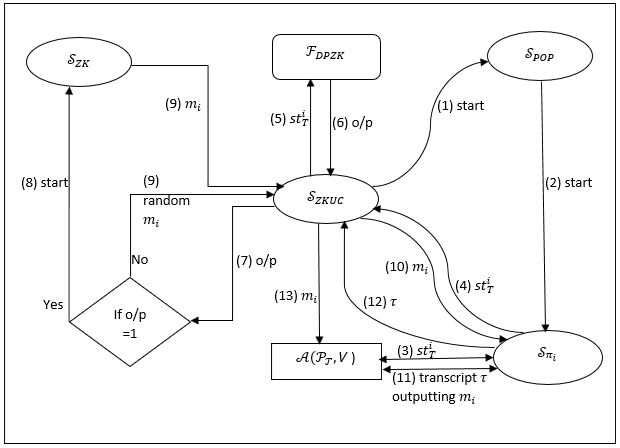
\includegraphics[width=\linewidth]{Diagram1.jpg}
		\caption{Simulation of the $i$th round}
		\label{fig:simulation}
	\end{figure}
	
	At $i$th round $\Sim$ on input $\stmt$ does the following: 
	\begin{itemize}
		\item $\Sim$ calls $\Sim_P$ on input $\stmt$, which internally calls $\Sim_{\pi_i}$ om input $\stmt$. 
		
		\item $\Sim_{\pi_i}$ starts interacting with the adversary and extracts $st^i_T$.
		
		\item 
		\begin{itemize} 
			\item $\Sim$ on first round, i.e., i=1 calls $\IF{DPZK}$ and checks whether corrupt provers are using correct shares of the witness or not, and stores state {\bf true} if $\IF{DPZK}$ outputs 1, else stores {\bf false}.
			\item If $i \neq 1$ $\Sim$ checks whether the extracted witnesses at the $i$th round is consistent with the prior rounds witnesses. if yes then sets state {\bf true}, else {\bf false}.
		\end{itemize}
		%\item $\Sim$ calls $\Sim_P$ to get the random $r_1$ which is going to be used before the next round to update the provers states.
		\item If state of $\Sim$ is {\bf true}, then $\Sim$ calls $\Sim_{ZK}$ on input $\stmt$ and gets the output $m_i$, and if state of $\Sim$ is {\bf false}, then $\Sim$ picks a random $m_i$.
		
		%\item $\Sim$ calls $\Sim_{ZK}$ on input $\stmt$ and feeds $r_1$ to get $m_{1}$ as the first round message to the verifier.
		\item $\Sim$ feeds $m_i$ as the output of $\IF{\Exec_{\pi_i}}$ to the simulator $\Sim_{\pi_i}$ and gets a transcript of the interaction among the provers, which is indistinguishable from the actual execution of $\pi_i$.
		\item Finally $\Sim$ sends $m_i$ to the verifier.
		\item and gets challenge $r$ from the verifier.
		%\item Then $\Sim$ calls $\Sim_{P}$, which calls $\Sim_{\pi_1}$ on input $(\stmt, \st^0_T , m_{1})$ and gets $\tau_{1}$.
		%\item $\Sim$ sends $m_1$ to the verifier, and gets the response $r_1$, a random challenge (honest verifier).
		%\item $\Sim$ updates the states of the adversarial provers i.e. $\st^i_T = (\st^{i-1}_T, r_i)$ $\forall i>0$.
		%\item $\Sim$ calls $\Sim_P$ to get the random $r_i$, for all $1<i <R$.
		%\item $\Sim$ calls $\Sim_{ZK}$ on input $\stmt$ and feeds $(r_1, \ldots, r_i)$ to get $m_i$ for all $1<i<R$.
		%\item Then $\Sim$ calls $\Sim_{P}$, which calls $\Sim_{\pi_{i}}$ on input $(\stmt, \st^{i-1}_T , m_{i})$ and gets $\tau_{i}$ $\forall i>0$. 
		%\item $\Sim$ keeps repeating the above steps and stops when $i=\round - 1$. 
	\end{itemize}
	$\Sim$ outputs $\Gamma = \{\tau_1, m_1 ,r_1, \ldots, \tau_{\round}, m_{\round}, r_{\round} \}$ 
	
	\noindent If corrupt parties used the correct shares of the input, then the transcript is accepting. Therefore, $\Gamma$ is indistinguishable from a transcript $\Gamma'$ of actual execution of the complete protocol where corrupt provers did not deviate from there shares of the witness, where
	Let $\Gamma' = \{\tau'_1, m'_1 ,r'_1, \ldots, \tau'_{\round}, m'_{\round}, r'_{\round} \}$ be a transcript of an actual execution of the protocol.
	
	Furthermore, if corrupt provers used some input which either not correct shares of the witness or inconsistent states, that leads to rejection, in that case; also the simulated transcript is indistinguishable from the actual execution of the complete protocol.
	%Claim: for any $\ppt$ algorithms, the distribution of $\Gamma$ and $\Gamma'$ is a negligible distance apart.
	To prove the above claim consider the following hybrid: 
	
	$\Gamma_0 = \{\tau'_1, m_1 ,r_1, \ldots, \tau'_{\round}, m_{\round}, r_{\round} \}$
	
	$\Gamma \approx \Gamma_0 : $ Since the simulator of privacy among the provers outputs indistinguishable transcripts in every round and all the executions in each round is independent as the verifier sends random challenges in each round which is used to update the states of the provers, $\tau_1 \approx \tau'_1$ and $\tau_2 \approx \tau'_2 \implies \{\tau_1, \tau_2\} \approx \{\tau'_1, \tau'_2\}$. Hence, $\Gamma \approx \Gamma_0$.
	
	$\Gamma_0 \approx \Gamma': $ If not then there is a $\ppt$ distinguisher $\calD$ for $\Gamma_0$ and $\Gamma'$. There is an easy to construct a $\ppt$ distinguisher, which can distinguish whether a transcript is an actual prover verifier interaction or generated by the simulator $\Sim_{ZK}$, using $\calD$, which breaks the zero-knowledge property of the protocol. Hence, $\Gamma_0 \approx \Gamma'$.
	
	Therefore, $\Gamma \approx \Gamma'$.
	
	That implies $\innp{\Pi}{\verifier}$ has zero-knowledge under $t$-collusion property.
	
	\textbf{case 2:} Let $\innp{\Pi}{\verifier}$ has $t$-ZKUC property.
	
	Then it is evident that $\innp{\Pi}{\verifier}$ has $ZK$; it is just a particular case of $t-ZKUC$, when $t=0$.
	
	It is easy to build a simulator $\Sim_P$ from the ZKUC simulator $\Sim$: $\Sim_P$ executes all the steps of $\Sim$ similarly, but for verifier's query, $\Sim_P$ picks $r$ uniformly at random and proceeds.
	%Now we will prove that $\innp{\Pi}{\verifier}$ has $t$-privacy among provers property. 
	This completes the proof.
%If not, let there is a set $T\subseteq [\Num]$ of size $\leq t$ for which during the interaction among the provers, adversary corrupting provers in $T$ learns a function $h(\wit)$ which can not be computed by the advesary i.e. $h(\wit)$ cannot computed using $\stmt, \wit_T, m, z$. Therefore $\verifier^*$ is learning $h(w)$, which he is not supposed to learn. That imples $\innp{\Pi}{\verifier}$ does not have ZKUC property, contradiction.

%Therefore $\innp{\Pi}{\verifier}$ has $t$-privacy among provers and zero-knowledge property.
\end{proof}


\paragraph{Efficiency measures}
In addition to the efficiency measures used for single-prover protocols, $\DPZK$ protocols are also measured in terms of the complexity and number of rounds involved in the communication between the provers. We now state all the efficient measures used to quantify a $\DPZK$ protocol.
\begin{enumerate}
\item Complexity of $\Pi$: The protocol $\Pi$ is measured in terms of the following complexities:
\begin{itemize}
\item \textit{computation} complexity for the provers
\item total \textit{communication} complexity between the provers
\item number of \textit{rounds} of communication between the provers
\end{itemize}
\item Verifier complexity
\item Proof size
\end{enumerate}

\subsection{Circuit share complexity}
Consider a relation where the witness is \textit{partitioned} among the provers in the $\DPZK$ setting. We define a new notion of efficiency for a $\DPZK$ protocol which would become a prominent efficiency measure for a class of real-world applications.
Let \textit{shared circuit} denote the part of the circuit representing the relation whose wire values are functions of inputs from more than one prover. 
We introduce the notion of \textit{circuit share complexity} to denote the size of this shared circuit.
Consider the class of applications where hashes (or any other commitment) of data from different parties are stored on a blockchain and a zero-knowledge proof has to be generated on an aggregation of all the data. This could be: 
\begin{enumerate}
\item Finance network: different bank account holders proving to a loan provider that the sum of their account balances is greater than the required threshold.
\item Trade logistic network: different logistic providers proving to a customer or regulator that the average delay of shipment along a particular route is less than a specified time.
\end{enumerate}
In all the applications in this class, each party participating in the aggregation first proves the \textit{relevance} of his/her data before they all run a protocol to prove the aggregated value on their data together. The proof of relevance involves proving that the data corresponds to a commitment in the blockchain network by proving the knowledge of the opening of a commitment in the blockchain. 
For instance, when using verifying a hash commitment within a proof system which works with circuit representation of the relation, the proofs of relevance i.e. the hash verifications of the individual data take up most of the gates in the circuit. But each such verification rely only on data from a single party. The aggregation does involve data from multiple parties but this step requires a relatively smaller number of gates. Hence, the circuit share complexity is very small for such applications, compared to the total size of the circuit. A DPZK protocol with its complexities proportional to the circuit share complexity instead of the total circuit complexity can attain major savings for such applications.
In general, the compatibility of the commitment with function representation of the proof system plays a part in the above discussion. We will discuss the relevant work on this compatibility in more detail in Section \ref{sec:relatedwork}.

Looking ahead, the complexity of the interaction between the provers in our DPZK protocol will be linear only in the circuit share complexity of the circuit predicate to be proven, and not in the \textit{total} size of the circuit. 
 
\subsubsection{Discussion}
Discussion on the definition.

Discussion on the sharing the witness among the parties instead of partitioning the witness.
\begin{itemize}
\item DPZK definitions are cleaner this way than having partitions?
\item The circuit size does not have to take into account the number of provers.
\end{itemize}

%\subsection{Construction step 1: The introduction of homomorphic commitments}
%
% -- some technical description of the techniques, and how "commitment oracle"
%helps in realizing DPZK
%
%\paragraph{Note} If we did not use homomorphic commitment we get +poly(secp).N protocol.
